% !Mode:: "TeX:UTF-8"
\section{主要研究内容}

本课题将研究软件服务和业务服务的不确定性决策,首先建立服务不确定性决策模型,基于此模型采用软件服务实现不确定性决策,然后上升到业务服务的不确定性决策。通过对软件服务的不确定性仿真,进而将业务服务的不确定性决策应用在海运物流的业务中,从而完成本课题。

因此,将要研究的内容主要分为~5~个部分,它们之间的逻辑关系如图~\ref{main_content}~所示。

\begin{figure}[htbp]
    \centering
    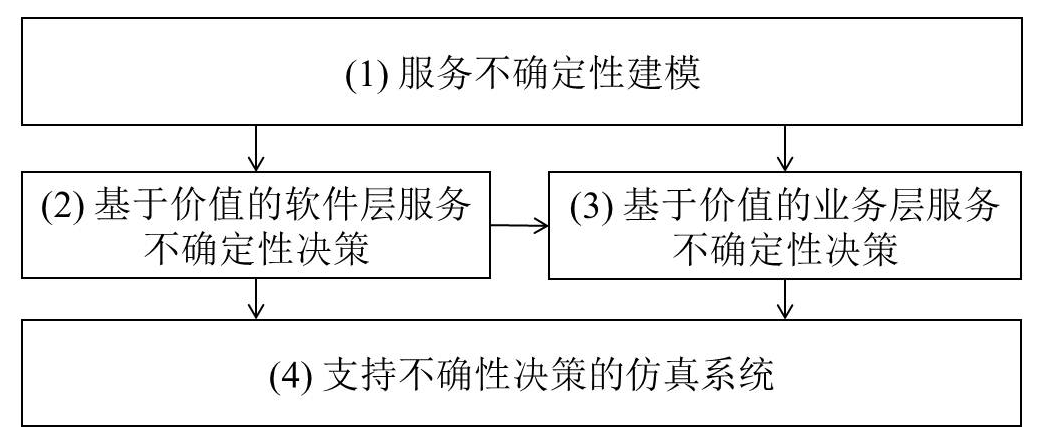
\includegraphics[width = 0.5\textwidth]{main_content}
    \caption{项目研究内容之间的逻辑关系}\label{main_content}
    \vspace{-1em}
\end{figure}

(1)~基于价值的服务不确定性建模

针对软件服务,分别识别服务执行过程中可能面临的多种不确定性,对服务不确定性进行分类,并提出不确定性触发关系图~(Uncertainty Triggering Graph, UTG)~以描述多种不确定性事件之间可能存在的触发关系。同时,识别每种不确定性事件发生后可能的决策动作并将其分类,由于采用不同的动作其所获得的价值是同的,因此建立其收益/成本度量模型,来衡量不同决策动作之间的优劣,并研究决策出最优的动作。

(2)~基于MDP的软件服务不确定性决策

根据服务执行中发生的具体不确定性,研究相应的不确定性触发关系图~(UTG)~的动态生成方法。提出基于动态~UTG~的不确定性影响范围及代价分析方法。识别优化目标(服务成功概率最大、时间延迟最小、成本最低),建立基于~Markov~决策过程~(MDP)~的不确定性优化决策模型并加以求解,生成对当前服务方案的最优改进策略。研究面向最小代价的运行时服务流程重组算法。

(3)~基于XX的业务服务不确定性决策



(4)~不确性决策的仿真系统

针对软件层面的服务不确定性,开发一个服务不确定性决策原型系统。此系统将融入基于~Markov~决策过程的服务不确定性决策方法,将不确定性事件采用某种随机策略产生,使得服务执行至故障状态,采用不确定性决策算法对故障状态的服务流程进行最优动作的决策,使得服务方案得以继续执行。

针对服务不确定性算法(基于~MDP~的服务自适应算法),采用传统的单步决策(贪心决策)与之进行对比,通过对比本课题的算法和传统算法的价值差(价值衡量),以及算法本身(时间复杂度和空间复杂度),从而证明本课题算法的有效性。

(5)~不确性决策在海运物流中的应用验证

针对业务层面的服务,在以上两个软件层面的不确定性决策研究的基础之上,通过具体的海运业务示例,建立海运业务的不确定性的分类,研究针对其具体业务的决策方法,以及其不确定性事件之间可能存在的触发关系,建立其服务不确定性决策模型,并自动求解其针对当前业务执行状态的最优(成本最低/价值最高)策略。

针对业务层面的不确定性,通过海运业务示例,提供海运服务接口和产生海运不确定性事件,对比其决策结果与传统人工决策结果,并对比其自动化决策效率和传统的人工决策效率之间的差值,将证明其决策效果的有效性和自动化决策的高效性。

针对海运物流业务层面,开发一个具备海运物流不确定性事件自动化决策的应用系统。此系统将建立海运业务的具体业务执行流程,用~Web Service~提供海运业务的服务接口,从而使得海运业务IT化。系统将采用服务不确定性决策算法,针对业务层面进行服务不确定性决策,使之具备海运业务不确定性的自动决策功能。
